
% =====================================================================
%  plantilla Jinja2 de mineria_academica
%  ------------------------------------------------------------------
%  Render :  latex_gen.generar_tex()  ->  salida/<tema>.tex
%  Compile:  pdflatex <tema>.tex  (dos veces: la 2a resuelve el indice)
%
%  DOS TRAMPAS DE JINJA + LATEX, ya resueltas aqui:
%    1) {#1}  (parametro de macro de LaTeX) lo lee Jinja como inicio de
%       comentario  ->  las definiciones \newcommand van en  raw .
%    2) %}    (escape de porcentaje de LaTeX) lo lee Jinja como cierre de
%       bloque   ->  en el cuerpo se usa la macro \pcento.
%  Paquetes: solo los base de cualquier instalacion (article, inputenc,
%  fontenc, geometry, graphicx, hyperref) para que compile en TeX minimo.
% =====================================================================
\documentclass[11pt,a4paper]{article}

% ---------------------------------------------------------------------
%  Paquetes
% ---------------------------------------------------------------------
\usepackage[utf8]{inputenc}     % acentos y enye correctos en Windows y Linux
\usepackage[T1]{fontenc}
\usepackage[margin=2.5cm]{geometry}
\usepackage{graphicx}           % \includegraphics de los PNG
\usepackage{hyperref}           % enlaces clicables

% Opcionales, descomenta si los tienes (no hacen falta para este informe):
\usepackage[spanish]{babel}   % requiere el idioma espanol instalado
% \usepackage{fancyhdr}         % encabezado y pie personalizados
% \usepackage{booktabs}         % \toprule / \midrule / \bottomrule
% \usepackage{enumitem}         % listas compactas
% \usepackage{xcolor}           % colores en los enlaces (requiere hyperref)

% ---------------------------------------------------------------------
%  Configuracion de hyperref
% ---------------------------------------------------------------------
\hypersetup{
  hidelinks,                    % enlaces sin color: no hace falta xcolor
  breaklinks=true,
  pdftitle={ Data Warehouse y OLAP },
  pdfauthor={ Generado automaticamente por mineria\_academica },
  pdfsubject={Informe de Data Warehouse y OLAP generado por mineria\_academica}
}

% Numeracion simple y parrafos sin sangria: informe tecnico, no carta.
\pagestyle{plain}
\setlength{\parindent}{0pt}
\setlength{\parskip}{6pt}
\sloppy                        % evita cajas desbordadas con textos largos


% ---------------------------------------------------------------------
%  Macros propios
%  Van dentro de un bloque raw porque Jinja interpretaria {#1} como el
%  inicio de un comentario y la plantilla dejaria de funcionar.
% ---------------------------------------------------------------------
\newcommand{\tema}[1]{\textbf{\textit{#1}}}
\newcommand{\nombrearchivo}[1]{\texttt{#1}}
\newcommand{\pcento}{\%}

\begin{document}

% =====================================================================
%  PORTADA
% =====================================================================
\begin{titlepage}
  \centering
  \vspace*{2.0cm}

  {\Large\textsc{Informe generado automáticamente}\par}
  \vspace{0.7cm}
  {\huge\bfseries Data Warehouse y OLAP\par}
  \vspace{0.4cm}
  {\large Analisis documental con TF-IDF y similitud del coseno\par}

  \vspace{1.8cm}

  \begin{minipage}{0.92\textwidth}
    \hrule
    \vspace{0.4cm}
    {\small
    \textbf{Tema:} \tema{ data\_warehouse }\\[4pt]
    \textbf{Documentos analizados:} 1\\
    \textbf{Documentos relevantes:} 1\\
    \textbf{Umbral de relevancia acumulado:} 80\pcento\\
    \textbf{Mínimo de resultados sin umbral:} 1\\
      	extbf{Fecha de generación:} \today
    \par}
    \vspace{0.4cm}
    \hrule
  \end{minipage}

  \vfill

  {\small mineria\_academica --- Python + scikit-learn + matplotlib + Jinja2\par}
  {\footnotesize
   Proceso 100\pcento\ local: sin APIs externas, sin claves y sin conexión
   a internet.\par}
\end{titlepage}

\tableofcontents
\newpage

% =====================================================================
%  1. INTRODUCCION
% =====================================================================
\section{Introducción}
\label{sec:introduccion}

Este informe corresponde al tema \tema{ Data Warehouse y OLAP } dentro del
proyecto \textit{ mineria\_academica }, una herramienta de minería académica que
opera completamente de forma local. El proceso seguido es el siguiente:

\begin{enumerate}
  \item \textbf{Ingesta}: lectura de los archivos \texttt{.pdf} y
        \texttt{.txt} de la carpeta \texttt{documentos/}.
  \item \textbf{Relevancia}: vectorización \textit{TF-IDF} de cada documento
        y comparación con la consulta del tema mediante similitud del coseno.
  \item \textbf{Clasificación}: asignación de cada documento al tema más
        cercano usando las consultas como centroides.
  \item \textbf{Informes}: generación de este documento en \LaTeX{} y de los
        gráficos correspondientes en PNG.
\end{enumerate}

Todo el proceso es determinista y reproducible: no depende de servicios
externos, no requiere GPU y puede ejecutarse sin conexión a internet.

\subsection{Consulta booleana utilizada}
\label{sec:query}

La siguiente expresión booleana está preparada para Google Scholar y es la que
se empleó como centroide para medir la relevancia de los documentos:

\begin{quote}
\small\ttfamily
("data warehouse" OR "data warehousing" OR OLAP) AND ("dimensional modeling" OR "star schema" OR "snowflake schema" OR "fact table" OR "data mart" OR ETL)
\end{quote}

Al eliminar los operadores \texttt{OR}, \texttt{AND} y \texttt{NOT} queda el
núcleo semántico de la búsqueda, que se convierte en vector \textit{TF-IDF} y
se compara con cada documento mediante la similitud del coseno.

La selección es \textbf{acumulativa}: los documentos se ordenan por relevancia
descendente y se conservan hasta alcanzar un umbral del
80\pcento. Si ni sumando todos los documentos se alcanza
dicho umbral, el sistema devuelve igualmente los 1
documentos más cercanos y lo advierte por consola, priorizando obtener un
resultado débil antes que dejar al usuario sin salida.

\subsection{Interpretación de la puntuación}

La puntuación mostrada es la similitud del coseno multiplicada por 100. Como
el coseno compara un documento (a menudo de varias páginas) con una consulta
breve, los valores absolutos suelen ser bajos y lo significativo es el
\textbf{orden}: los primeros documentos de la lista~\ref{sec:relevantes} son
los que más comparten léxico con la consulta del tema.

% =====================================================================
%  2. DOCUMENTOS RELEVANTES
% =====================================================================
\section{Documentos relevantes}
\label{sec:relevantes}

Se identificaron 1 documento(s) relevante(s) de los
1 analizados, ordenados de mayor a menor relevancia:

\begin{enumerate}
\setlength{\itemsep}{6pt}
\renewcommand{\labelenumi}{\arabic{enumi}.}
  \item \nombrearchivo{ paper.txt } --- \textbf{ 7.88\pcento}
\end{enumerate}

\begin{center}
\begin{tabular}{r p{8.5cm} r}
\hline
\textbf{\#} & \textbf{Documento} & \textbf{Relevancia} \\
\hline
1 & paper.txt & 7.88\pcento \\
\hline
\end{tabular}
\end{center}


% =====================================================================
%  3. GRAFICO
% =====================================================================
\section{Gráfico de relevancia}
\label{sec:grafico}

\begin{figure}[htbp]
  \centering
  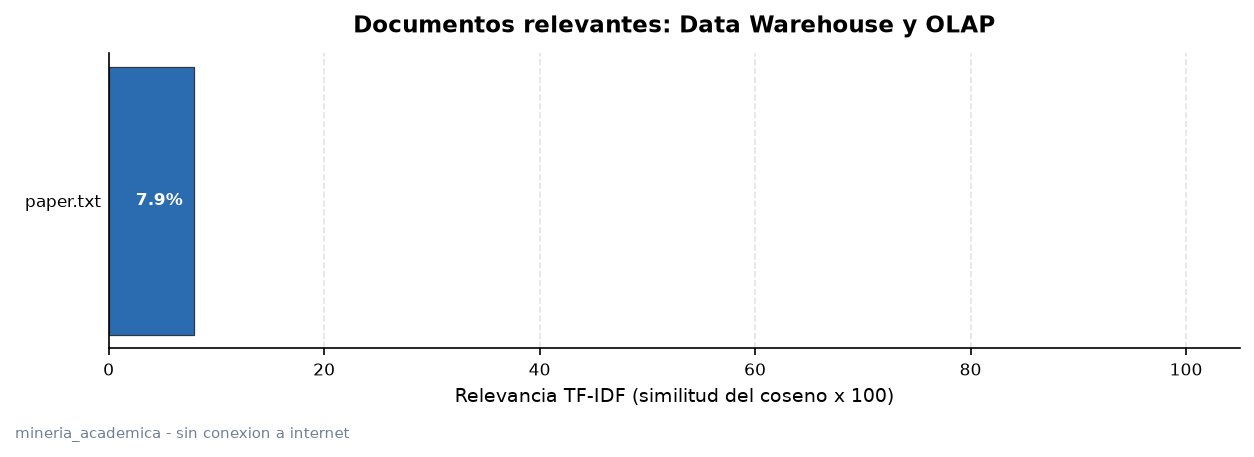
\includegraphics[width=0.95\textwidth]{ grafico_data_warehouse.png }
  \caption{ Relevancia TF-IDF de los documentos frente a la consulta de Data Warehouse y OLAP. }
  \label{fig:relevancia}
\end{figure}

La figura~\ref{fig:relevancia} muestra el porcentaje de relevancia de cada
documento frente a la consulta del tema. Las barras más largas corresponden a
los documentos que comparten mayor número de términos significativos con la
búsqueda booleana de la sección~\ref{sec:query}.


% =====================================================================
%  4. EJEMPLO
% =====================================================================
\section{Ejemplo}
\label{sec:ejemplo}

A continuación se reproduce un fragmento de
\nombrearchivo{ paper.txt } como ejemplo de la evidencia
recuperada para este tema:

\begin{quote}
\small
Knowledge discovery in databases uses data mining algorithms. The KDD process includes data preparation, modeling and evaluation.
\end{quote}


% =====================================================================
%  5. CONCLUSIONES
% =====================================================================
\section{Conclusiones}
\label{sec:conclusiones}

\begin{itemize}
\setlength{\itemsep}{4pt}
  \item La consulta booleana de \tema{ Data Warehouse y OLAP } recupera
        1 documento(s) de los 1
        analizados en la corpus local.
  \item El método basado en \textit{TF-IDF} y similitud del coseno es
        totalmente local y reproducible, sin depender de servicios externos,
        claves de API ni conexión a internet.
  \item La clasificación automática por centroides permite organizar la
        biblioteca por tema sin intervención manual, y marca como
        \tema{sin\_clasificar} los documentos con confianza insuficiente en
        lugar de asignarlos a la fuerza.
  \item El gráfico~\ref{fig:relevancia} junto con la tabla de la
        sección~\ref{sec:relevantes} facilita la priorización de lecturas.
\end{itemize}

\subsection*{Siguientes pasos sugeridos}

\begin{itemize}
\setlength{\itemsep}{3pt}
  \item Ampliar la carpeta \texttt{documentos/} con nuevas búsquedas
        ejecutadas en Google Scholar a partir de las consultas de la
        sección~\ref{sec:query}.
  \item Ajustar el punto de corte con la opción \texttt{--umbral} y el mínimo
        de resultados con \texttt{--minimo} de \texttt{main.py}.
  \item Reejecutar el pipeline completo con \texttt{python main.py --todo}
        y consultar los resultados con el modo de preguntas:
        \texttt{python main.py --interactivo-qa}.
\end{itemize}

\vfill
\begin{center}
\small
\textit{Documento generado automáticamente por mineria\_academica.\\
No requiere GPU, ni APIs externas, ni conexión a internet.}
\end{center}

\end{document}
